\section{Introduction}
\label{sec:intro}

Facial emotion recognition (FER)~\cite{Ko18} is not only an interesting in our daily life, 
but also important in the realm of artificial intelligence and computer vision. 
In this short proposal, 
we aim to leverage several deep neutral networks to analyze and interpret different human facial emotions.

The structure of this report is arranged as follows. 
% \Cref{sec:related} contains the related work of our research. 
In \Cref{sec:approach}, 
we provide the datasets we used, 
the model architecture we implemented, 
and preliminary evaluation results of our model. 
Our code and supplementary material is available at \url{https://github.com/werywjw/SEP-CVDL}.

\begin{figure*}
  \resizebox{\textwidth}{!}{
    \begin{ganttchart}[
      % hgrid,
      vgrid,
      time slot format=isodate,
      x unit=0.3cm, 
      y unit title=0.9cm,
      y unit chart=0.45cm,
      bar height=0.35,
      bar top shift=0.2,
      group right shift=0,
      group top shift=0.1,
      group height=.3,
      group peaks width={0.2},
      milestone left shift=0.5,
      milestone right shift=0.5,
      title label font=\bfseries\Large
  ]{2023-12-21}{2024-02-23}
      \gantttitlecalendar{year, month} \\
      \ganttbar[bar/.append style={fill=LMUGreen}]{Data Collecting \& Processing}{2023-12-21}{2024-01-10} \\
      \ganttbar[bar/.append style={fill=LMUGreen}]{Model Implementing}{2023-12-30}{2024-01-20} \\
      \ganttbar[bar/.append style={fill=LMUGreen}]{Model Training \& Validating}{2023-12-30}{2024-01-20} \\
      \ganttbar[bar/.append style={fill=LMUGreen}]{Report Writing}{2024-01-04}{2024-01-16} \\
      \ganttgroup[bar/.append style={fill=LMUGreen}]{Preliminary Report}{2023-12-21}{2024-01-17} \\
      % \ganttmilestone{Deadline 1}{2024-01-18} \\
      \ganttbar[bar/.append style={fill=Orange}]{Explainable AI}{2024-01-05}{2024-01-18} \\
      \ganttbar[bar/.append style={fill=Orange}]{Model Fine-Tuning}{2024-01-05}{2024-02-07} \\
      \ganttgroup[bar/.append style={fill=Orange}]{Presentation}{2024-01-05}{2024-02-07} \\
      % \ganttmilestone{Deadline 2}{2024-02-08} \\
      \ganttbar[bar/.append style={fill=cvprblue}]{Report Writing}{2024-01-17}{2024-02-22} \\
      \ganttgroup[bar/.append style={fill=cvprblue}]{Final Submission}{2024-01-19}{2024-02-22} \\
      % \ganttmilestone{Deadline 3}{2024-02-23}
      % \ganttlink{elem3}{elem8}
      % \ganttlink{elem2}{elem3}
      % \ganttlink{elem2}{elem4}
      % \ganttlink{elem4}{elem5}
  \end{ganttchart}
  }
  \caption{Overview of the time schedule for the final project}
  \label{fig:schedule}
\end{figure*}

%-------------------------------------------------------------------------
% All authors will benefit from reading Mermin's description of how to write mathematics:
% \url{http://www.pamitc.org/documents/mermin.pdf}.

% Short captions should be centered.



% \begin{figure*}
%   \centering
%   \begin{subfigure}{0.68\linewidth}
%     \fbox{\rule{0pt}{2in} \rule{.9\linewidth}{0pt}}
%     \caption{An example of a subfigure.}
%     \label{fig:short-a}
%   \end{subfigure}
%   \hfill
%   \begin{subfigure}{0.28\linewidth}
%     \fbox{\rule{0pt}{2in} \rule{.9\linewidth}{0pt}}
%     \caption{Another example of a subfigure.}
%     \label{fig:short-b}
%   \end{subfigure}
%   \caption{Example of a short caption, which should be centered.}
%   \label{fig:short}
% \end{figure*}

\section{Approach}
\label{sec:approach}

\subsection{Dataset Aquisition and Processing}
Firstly, 
for all the image data from the training dataset RAF-DB\footnote{\url{http://www.whdeng.cn/raf/model1.html}}~\cite{li2017reliable,li2019reliable}, 
we filter out neutral instances from the original dataset, 
the emotion labels are denoted as 1 (Surprised), 2 (Fearful), 3 (Disgusted), 
4 (Happy), 5 (Sad), and 6 (Angry) for simplicity 
(Our first dataset is downloaded from \url{https://www.kaggle.com/datasets/shuvoalok/raf-db-dataset/code} with the addition csv file to their labels). 
The test result in \Cref{fig:result} is also aggregated from this specific dataset.
To transform and resize the images to \texttt{(64,64)}, 
we convert the images to greyscale with three channels as our original CNN is designed to work with three-channel inputs. 
Also, we randomly flip the images horizontally with a default 50\% chance. 
This kind of augumentation helps in making the model more robust to orientation changes and thus improve the generalization ability. 
Our training dataset is aggregated from CK+~\cite{LuceyCKSAM10}.

\subsection{Model Architecture}
We implemented an emotion-classification model with four convolution layers. 
Following each convolutional layer, 
batch normalization is applied. 
This stabilizes learning by normalizing the input to each layer. 
Then three linear layers are applied to extract features to the final output. 
We also add a \texttt{dropout} layer to prevent overfitting. 
The activation function used after each layer is Rectified Linear Unit (ReLU), 
since it introduces the non-linearity into the model, 
allowing it to learn more complex patterns. 
In order to find the best hyperparameter configuration (see \cref{tab:hyper} for details) of the model, 
we utilize the parameter grid from sklearn~\footnote{\url{https://scikit-learn.org/stable/modules/generated/sklearn.model_selection.ParameterGrid.html}}. 

% model comparison, e.g., SVM try, also VGG
% specific dataset comparison, e.g., RAF-DB & FER+
% Create table for results 

\begin{table}
    \centering
    \begin{tabular}{@{}lc@{}}
      \toprule
      Hyperparameter & Configuration \\
      \midrule
      Learning rate & \{0.1, 0.01, 0.001, 0.0001\}  \\
      Batch size & \{8, 16, 32, 64\} \\
      Dropout rate & \{0.5\} \\
      Epoch & \{10, 20, 30\} \\
      Early stopping & \{\texttt{True}, \texttt{False}\} \\
      Patience & \{5\} \\
      \bottomrule
    \end{tabular}
    \caption{Explored hyperparameter space for our model}
    \label{tab:hyper}
  \end{table}

\subsection{Preliminary Results}

For evaluation, we use the metric accuracy. 
The loss function is cross entropy, which is typically for multi-class classification. 
The main results of our experiment with respect to loss and accuracy is depicted in \Cref{fig:result}.

\begin{figure}[t]
  \centering
  % \fbox{\rule{0pt}{2in} \rule{0.9\linewidth}{0pt}}
   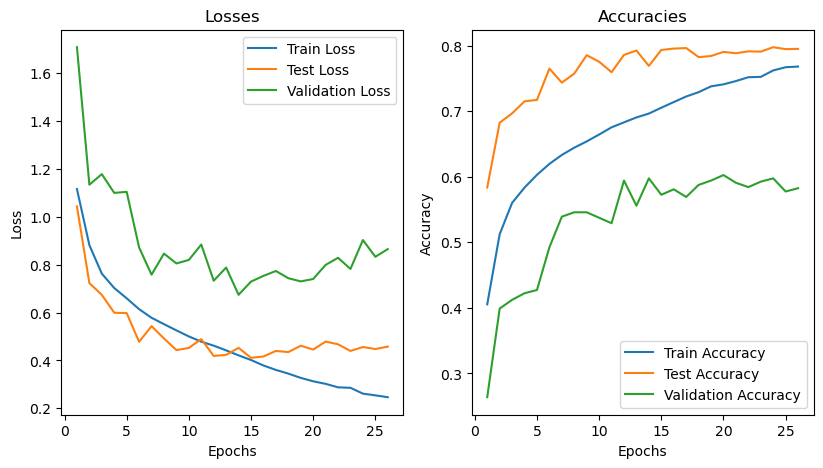
\includegraphics[width=0.95\linewidth]{output.png}
   \caption{Empirical results in terms of the loss and accuracy on differen training epochs}
   \label{fig:result}
\end{figure}

\section{Optimization Strategies}
In the coming weeks, 
we 

\subsection*{Author Contributions}
\label{sec:author}
% see https://arxiv.org/pdf/2005.14165.pdf page42
Equal contributions listed by alphabetical order of surnames. 
Every author did the literature research and contributed to the writing of the paper. 
An overview of our time schedule for the entire final project is given in \Cref{fig:schedule}. 

\begin{itemize}
  \item \textbf{Tanja Jaschkowitz} implemented the model architecture, training infrastructure, 
  \item \textbf{Leah Kawka} collected the training data, prepared dataprocessing, implemented augmentation, Explainable AI \& Video-green square
  \item \textbf{Mahdi Mohammadi} implemented the 
  \item \textbf{Jiawen Wang} implemented the model architecture, training infrastructure, and optimization strategies. 
  In the specific wrting part, she also checked and aggereated this report from other team members.
\end{itemize}

\section*{Acknowledgements}

We are deeply grateful to our advisors \textbf{Johannes Fischer} and \textbf{Ming Gui} for their helpful and valuable support during the entire semester. 
We also thank \textbf{Prof. Dr. Björn Ommer} for providing this interesting practical course.